

\chapter{Stand der Wissenschaft und Technik}\label{cha:2}

Zur Abbildung geeigneter Welleneigeschaften in einer Messkabine, die selbst ebenfalls möglichst wenig Beeinflussung durch äußere Felder erfährt, ist ein grundlegendes Verständnis elektrischer und magnetischer Felder, sowie deren Ausbreitung im Raum und Interaktion mit unterschiedlichen Grenzschichten notwendig. Weiterhin soll die Schirmdämpfung als zu messende Größe der CNT-Folien allgemein betrachtet werden, sodass im Anschluss daran verschiedene Möglichkeiten der Messung vorgestellt werden können. \par
\vspace{\linespace}
Mithilfe der Theorie der Eigenschaften von Wellenfeldern wird dann aus betrachteten Messmethoden die ausgewählt, mit der sich die Anforderungen an die durchzuführende Vermessung von Schirmmaterialien bestmöglich erfüllen lassen. Die wissenschaftlichen Grundlagen dienen weiterhin als Basis für die Detailkonstruktion der Messkabine.


\section{Grundlagen elektromagenetischer Wellenfelder}\label{cha:2_Grundlagen}


Allgemein beschreibt ein Feld die Gesamtmenge aller Werte einer physikalischen Größe, die allen Punkten eines leeren oder stoffgefüllten Raumes zugeordnet sind, die sogenannte Feldgröße \cite{Spektrum.de_Feld}. Je nach Art der Feldgröße wird der allgemeine Feldbegriff in Skalarfeld 

\begin{equation}
    a(x,y,z, \ldots)    
\end{equation}


und Vektorfeld 

\begin{equation}
    \vec A(x,y,z,\ldots)
\end{equation}

unterteilt. Durch die Darstellung der Abhängigkeit von den Ortskoordinaten des Raumes wird deutlich, dass es sich bei einer Größe um ein Feld handelt. \par
\vspace{\linespace}
Die im Rahmen dieser Arbeit wichtigen Felder sind das elektrische und das magnetische Feld. Eine Beschreibung des Zusammenhanges zwischen der Feldursache und dem entstehenden Feld lässt sich in beiden Fällen mithilfe der Materialgleichungen und der Maxwell'schen Gleichungen vornehmen~\cite{EM_Schirmung}. Grundlegend lässt sich ein Feld jedoch auch ohne Kenntnis seiner Ursache beschreiben, sodass im Rahmen dieser Arbeit nicht explizit auf die Maxwell'schen Gleichungen eingegangen werden soll, da dies thematisch zu weit führen würde. 


\subsection{Elektrisches Feld}\label{cha:2_sub_Elektrisches_Feld}

Um das elektrische Feld mittels seiner Wirkungs zu beschreiben, wird eine Testladung in das Feld eingebracht, auf die daraufhin eine Kraft $\vec F_q(x,y,z,q)$ wirkt. Da die Kraft eine gerichtete Größe ist, muss die Beschreibung des elektrischen Feldes mittels eines Vektorfeldes beschrieben werden. Die Größe der Kraft ist abhängig von der eingebrachten Ladung. Um eine Veränderung des Feldes durch die Testladung auszuschließen, wird stattdessen eine infinitesimale Teilladung $dq$ zur Beschreibung des Feldes verwendet, was sich damit aus

\begin{equation}
    \vec E (x,y,z) = \frac{d\vec F_q(x,y,z,q)}{dq}
\end{equation}

ergibt. Der Differentialquotient $\vec E$ ist die elektrische Feldstärke \cite{EM_Schirmung}. \par
\vspace{\linespace}
Damit ist die Wirkung eines elektrischen Feldes beschrieben, jedoch noch nicht dessen Ursache. Nach dem sogenannten Satz des Hüllenflusses, dem ersten Maxwell'schen Gesetz, erfahren Ladungen nicht nur Beeinflussung durch ein elektrisches Feld, sondern sind auch dessen Ursache. Eine Beschreibung kann am einfachsten mithilfe eines Plattenkondensators erfolgen, dessen Plattenflächen $A_P$ senkrecht auf den Feldlinien eines elektrisches Feldes stehen und auf welche die Ladungen $+q$ und $-q$ genau so aufgebracht werden, dass im Inneren des Kondensators das äußere Feld kompensiert wird. Eine von der Fläche unabhängige Größe zur Beschreibung des elektrischen Feldes lässt sich wiederum durch den Differentielquotienten 

\begin{equation}
    \vec D(x,y,z) = \frac{dq}{dA_P} \cdot \vec n_A
\end{equation}

erhalten, der elektrischen Flussdichte $\vec D$ \cite{EM_Schirmung}. \par
\vspace{\linespace}

Da sowohl die Feldstärke als auch die Flussdichte das elektrische Feld beschreiben, gibt es in Abhängigkeit Materials, aus dem der felderfüllte Raum besteht, einen Zusammenhang zwischen beiden Größen, die sogenannte Dielektrizitätszahl oder Permittivität $\varepsilon$, die eine Materialeigenschaft ist. Es gilt

\begin{equation}
    \vec D = \varepsilon \cdot \vec E = \varepsilon_0 \varepsilon_r \cdot \vec E \qquad \quad \text{mit} \qquad \varepsilon_0 = 8,85419 \cdot 10^{-12} \; \si{\ampere\second\per\volt\per\meter}
    \label{eq:2_Materialgleichung_elektrisches_Feld}
\end{equation}

mit der Dielektrizitätszahl des leeren Raumes $\varepsilon_0$ und der relativen Dielektrizitätszahl $\varepsilon_r$ des betrachteten Materials \cite{EM_Schirmung}.


\subsection{Magnetisches Feld}\label{cha:2_sub_Magnetisches_Feld}

Wie auch die elektrische Feldstärke wird die magnetische Flussdichte indirekt beschrieben, d.h. über ihre messbare Kraftwirkung auf elektrische Ströme bzw. bewegte Ladungen. Dabei wird ein stromdurchflossener Draht der Länge $L$ so über einem Magnetfeld angeordnet, dass die messbare Kraft maximal wird. Um auch hier Rückwirkungen auszuschließen, wird eine differentielle Drahtlänge, die vom infinitesimal kleinen Strom $dI$ durchflossen wird, betrachtet. Mit des Differentialquotienten

\begin{equation}
    \vec B(x,y,z) = \frac{d^2 \vec F_L(x,y,z,L,I)}{dL \cdot dI}
\end{equation}

lässt sich die magentische Flussdichte, die sowohl vom Strom $I$ als auch von der Drahtlänge $L$ abhängt, aus der gemessenen Kraft ermitteln \cite{EM_Schirmung}. 
\par
\vspace{\linespace}
Analog zur Betrachtung elektrischer Felder lässt sich feststellen, dass Ströme nicht nur eine Kraftwirkung durch magnetische Felder erfahren, sondern auch deren Ursache sind. Dazu lässt sich ebenfalls ein einfaches Gedankenexperiment ähnlich der Betrachtung zur elektrischen Flussdichte durchführen: 
\par
\vspace{\linespace}
In einer Spule der Länge $L$ fließe ein Strom $I$, der genau so groß ist, dass durch die induzierte magnetische Flussdichte ein umgebendes äußeres Magnetfeld im Inneren der Spule verschwindet. Die Ausrichtung der Anordnung sei wiederum so erfolgt, dass der Strom $I$ maximal wird. Der erforderliche Strom ist abhängig von der Spulenlänge und deren Windungszahl $N_w$. Das Differential

\begin{equation}
    \vec H(x,y,z) = N_w \frac{dI(x,y,z,L)}{dL} \cdot \vec n_A
\end{equation}

beschreibt die magnetische Feldstärke, welche senkrecht auf der Spulenquerschnittsfläche steht \cite{EM_Schirmung}. 
\par
\vspace{\linespace}
Ebenso wie die elektrische Feldstärke und Flussdichte sind auch die beschreibenden Feldgrößen des magnetischen Feldes proportional zueinander und lassen sich über eine Materialkonstante, der sogenannten Permeabilität $\mu$, ineinander umrechnen:

\begin{equation}
    \vec B = \mu \cdot \vec H = \mu_0 \mu_r \cdot \vec H \qquad \quad \text{mit} \qquad \mu_0 = 4\cdot \pi \cdot 10^{-7} \; \si{\volt\second\per\ampere\per\meter}.
    \label{eq:2_Materialgleichung_magnetisches_Feld}
\end{equation}

Die relative Permeabilität $\mu_r$ ist ein Materialparameter und die Permeabilität des Vakuums $\mu_0$, ebenso wie $\varepsilon_0$, eine Naturkonstante \cite{EM_Schirmung}.
\par
\vspace{\linespace}
Eine Verknüpfung des elektrischen Feldes mit dem magnetischen kann über den ein einem Leiter hervorgerufenen Stromfluss erfolgen. Die verknüpfende Größe der erzeugten Stromdichte $\vec j$,

\begin{equation}
    \vec j = \sigma \cdot \vec E,
\end{equation}

ist dabei die Leitfähigkeit $\sigma$ des betrachteten Leitermaterials.


\subsection{Verhalten elektrischer und magnetischer Felder an Grenzflächen}

In den vorangegangenen \Abschnitten \ref{cha:2_sub_Elektrisches_Feld} und \ref{cha:2_sub_Magnetisches_Feld} wurde die Abhängigkeit der Flussdichte- und Feldstärkevektoren voneinandern mithilfe von Materialeigenschaften beschrieben. Breiten sich die Felder also entlang verschiedener Materialien mit unterschiedlichen Dielektrizitäten und Permeabilitäten aus, ändern sich beim Übergang zwangsläufig die Ausbreitungsbedingungen. Dies soll im Folgendes betrachtet werden, da das Verhalten der Felder an Materialgrenzflächen grundlegend für die Untersuchtung von Materialschirmen ist. 
\par
\vspace{\linespace}
Für die folgende Betrachtung sei angenommen, dass die untersuchte Grenzfläche relativ zum felderfüllten Raum eine allgemeine Lage aufweist und somit die jeweiligen Feldvektoren schräg auf die Grenzfläche auftreten (vgl. \Abb \ref{fig:2_Flussdichten_an_Grenzflaechen}). Weiterhin werden die Vektoren in der folgenden Untersuchung in ihre Normal- und Tangentialkomponente zur betrachteten Grenzfläche zerlegt, was jeweils durch die Indizes~$n$ und $t$ verdeutlicht wird. 

\begin{figure}[ht]
    \centering
    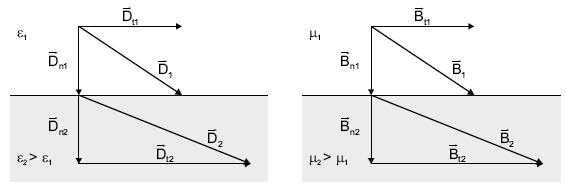
\includegraphics[width=0.75\textwidth]{Abbildungen/Kapitel2/Flussdichten_an_Grenzflaechen.png}
    \caption{Verhalten elektrischer und magnetischer Flussdichtevektoren an Grenzflächen von \mbox{Materialien} unterschiedlicher Dielektrizität bzw. Permeabilität}
    \label{fig:2_Flussdichten_an_Grenzflaechen}
\end{figure}

Beim Materialübergang von Flussdichtevektoren ist festzustellen, dass die Normalkomponenten an der Grenzfläche in beiden Materialien konstant sind (vgl. \Abb \ref{fig:2_Flussdichten_an_Grenzflaechen}) \cite{EM_Schirmung}.  

\begin{equation}
    \vec D_{n1} = \vec D_{n2}
\end{equation}
\begin{equation}
    \vec B_{n1} = \vec B_{n2}
\end{equation}


Aus den vorgestellten Materialgleichungen~\ref{eq:2_Materialgleichung_elektrisches_Feld} und \ref{eq:2_Materialgleichung_magnetisches_Feld} ergibt sich daraus für die Normalkomponenten der Feldstärke bei gleichbleibender Flussdichte zwangsläufig ein Sprung an der Grenzfläche im reziproken Verhältnis der Dielektrizitäten bzw. Permeabilitäten aufgrund der unterschiedlichen Materialeigenschaften. Somit gilt

\begin{equation}
    \vec E_{n1} = \frac{\varepsilon_2}{\varepsilon_1} \cdot \vec E_{n2} \\
\end{equation}
\begin{equation}
    \vec H_{n1} = \frac{\mu_2}{\mu_1} \cdot \vec H_{n2}
\end{equation}

für die Normalkomponenten der Feldstärken. Die Abbildung \ref{fig:2_Feldstaerken_an_Grenzflaechen} verdeutlicht dies. 

\begin{figure}[ht]
    \centering
    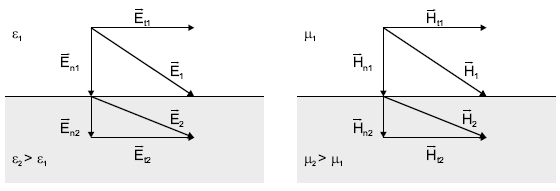
\includegraphics[width=0.75\textwidth]{Abbildungen/Kapitel2/Feldstaerken_an_Grenzflaechen.png}
    \caption{Verhalten elektrischer und magnetischer Feldstärkevektoren an Grenzflächen von \mbox{Materialien} unterschiedlicher Dielektrizität bzw. Permeabilität}
    \label{fig:2_Feldstaerken_an_Grenzflaechen}
\end{figure}

Betrachtet man die Feldursachen bzw. die beschreibenden Maxwell'schen Gleichungen wird offentlichtsicht, dass für die Vektoren der Feldstärke wiederum die Tangentialkomponente in beiden Materialien beim Übergang über die Grenzschicht gleich bleiben muss \cite{EM_Schirmung}. 

\begin{equation}
    \vec E_{t1} = \vec E_{t2}
\end{equation}
\begin{equation}
    \vec H_{t1} = \vec H_{t2}
\end{equation}

Mit einer ähnlichen Argumentation wie vorher kann gezeigt werden, dass damit für die tangentialen Komponenten der Flussdichtevektoren die Beziehungen

\begin{equation}
    \vec D_{t1} = \frac{\varepsilon_1}{\varepsilon_2} \vec D_{t2}
\end{equation}
\begin{equation}
    \vec B_{t1} = \frac{\mu_1}{\mu_2} \vec B_{t2}
\end{equation}

Damit gelten ebenfalls für die resultierenden Vektoren $\vec D_1$ und $\vec D_2$ bzw. $\vec B_1$ und $\vec B_2$ die Materialgesetze~\ref{eq:2_Materialgleichung_elektrisches_Feld} und \ref{eq:2_Materialgleichung_magnetisches_Feld}. Ein Sprung in den Materialeigenschaften äußert sich demnach in einer Brechung der resultierenden Feldlinien in Abhängigkeit der Verhältnisse $\varepsilon_1 / \varepsilon_2$ und $\mu_1 / \mu_2$, welche analog der Brechung von Licht beim Übergang in unterschiedliche optische Materialien veranschaulicht werden kann. Unter der Vorraussetzung isotroper Materialien hintsichtlicht Dielektrizität und Permeabilität gilt weiterhin, dass die resultierenden Flussdichte- und Feldstärkevektoren des elektrischen bzw. magnetischen Feldes in den jeweiligen Materialien kollinear sind und die gleiche Orientierung haben.

\par
\vspace{\linespace}

Für das Verständnis der Wirkungsweise von elektromagnetischen Schirmen ist dieses Verhalten von Feldern an Grenzflächen eine wichtige Grundvoraussetzung.




%Da Schirm für eindringende Wellen -> wichtig











\section{Wellenausbreitung}\label{cha:2_Wellenausbreitung}


\subsection{Entstehung einer elektromagnetischen Welle}\label{cha:2_sub_Entstehung_einer_Welle}

Die Entstehung einer elektromagnetischen Welle, ausgehend von einem Dipol beispielsweise, beruht auf der Wechselwirkung elektrischer und magnetischer Felder. Vereinfacht beschrieben führt ein Leitungsstrom zwischen einem Paar entgegengesetzter Ladungen (Dipol), zur Induktion eines Magnetfeldes, welches seinerseits wieder ein elektrischer Feld hervorruft. Im Verlauf des Ladungsausgleiches nimmt der Leitungsstrom und damit ebenfalls das Magnetfeld immer weiter ab. Diese zeitliche Änderung des magnetischen Feldes induziert gemäß des Induktionsgesetzes jedoch wiederrum ein elektrisches Feld entgegengesetzter Polarität, welches die beiden betrachteten Körper erneut auflädt. Der Leitungsstrom zwischen den Körpern fließt als Verschiebungsstrom\footnote{Verschiebungsströme beruhen im Gegensatz zu Leitungsströmen nicht auf dem Fluss von Ladungsträgern, sondern auf der zeitlichen Änderung elektrischer Felder und sind somit auch zwischen Raumpunkten ohne direkte Verbindung durch einen Leiter möglich. Der Begriff wurde durch J.C. Maxwell als Ergänzung zum Durchflutungsgesetz nach A.M. Ampére bekannt \cite{Feldtheorie_Begriffe}} wieder zurück, sodass ein geschlossener Stromkreis entsteht. Dieser periodische Schwingkreis führt zu einer Ausbreitung gekoppelter elektrischer und magnetischer Felder im Raum, was als elektromagnetische Welle bekannt ist. Für die Ausbreitung im Raum ist dabei kein umgebendes Medium notwendig \cite{EM_Schirmung}.
\par
\vspace{\linespace}
Wie in einem Schwingkreis aus Kapazität und Induktivität schwingt die im System vorhandene Energie zwischen den beiden unterschiedlichen Feldern hin und her. Im Verlauf der weiteren Betrachtungen wird, insofern nicht anders erwähnt, von einer harmonischen Schwingung ausgegangen.
\par
\vspace{\linespace}
Bei den sich im Raum ausbreitenden Feldern handelt es sich im reine Wirbelfelder mit in sich geschlossenen Feldlinien \cite{Feldtheorie_Begriffe} (siehe \Abb \ref{fig:2_Hertzscher_Dipol}). Für Magnetfelder ist dies ohnehin stets der Fall und da die elektrischen Felder aufgrund zeitlich veränderlicher magentischer Flüsse entstehen, treten diese ebenfalls in Form von Wirbelfeldern auf \cite{EM_Schirmung} \cite{Feldtheorie_Begriffe}. In der Nähe eines Dipols, also der Ursache der Welle, überlagern sich die Wirbelfelder mit den elektrischen Quellenfeldern, die aufgrund der Ladungsunterschiede auftreten \cite{EM_Schirmung}. 
\par
\vspace{\linespace}
Wird für die Betrachtung ein infinitesimal kleiner Dipol verwendet, trägt dieser die Bezeichnung Hertz'scher Dipol und stellt die einfachste Form einer Antenne dar. Zur theoretischen Betrachtung kann jede weitere, beliebige Antennenform aus Hertz'schen Dipolen superponiert werden \cite{EM_Schirmung}.
\par
\vspace{\linespace}
\begin{figure}
    \centering
    \begin{subfigure}[c]{0.4\textwidth}
        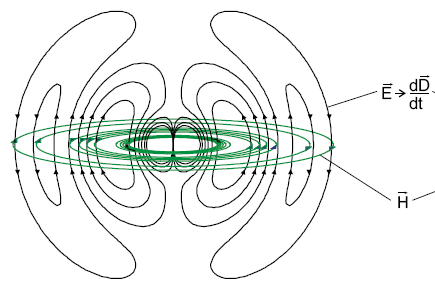
\includegraphics[width=\textwidth]{Abbildungen/Kapitel2/Hertz'scher_Dipol_A.png}
        \caption{}\label{subfig:2_Hertzscher_Dipol_A}
    \end{subfigure}
    \hspace{1cm}
    \begin{subfigure}[c]{0.4\textwidth}
        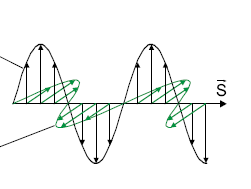
\includegraphics[width=\textwidth]{Abbildungen/Kapitel2/Hertz'scher_Dipol_B.png}
        \caption{}\label{subfig:2_Hertzscher_Dipol_B}
    \end{subfigure}
    \caption{Schematische Darstellung eines Hertz'schen Dipoles mit den umgebenden geschlossenen Wirbelfeldlinien in einer Momentdarstellung nach Quelle~\cite{EM_Schirmung}. Die dargestellte ebene Welle (b) bildet sich in ausreichend großer Entfernung von der Quelle aus.}
    \label{fig:2_Hertzscher_Dipol}
\end{figure}


\subsection{Feldverlauf in der Umgebung eines Dipols}\label{cha:2_sub_Feldverlauf_in_Umgebung_eines_Dipols}

Um die Charakteristik des umgebenden Feldes eines Dipols zu bestimmen ist es zielführend, die Komponenten der Feldstärken in Abhängigkeit des Abstandes zu betrachten. Da die Strahlungsfelder jeder Antenne endlicher Abmessung spärische Wellen sind \cite{Antenna_Theory}, ist weiterhin eine Betrachtung in Kugelkoordinaten $\left(r, \phi, \theta\right)$ zweckmäßig (siehe \Abb \ref{fig:2_Feldverlauf}). 

\begin{figure}
    \centering
    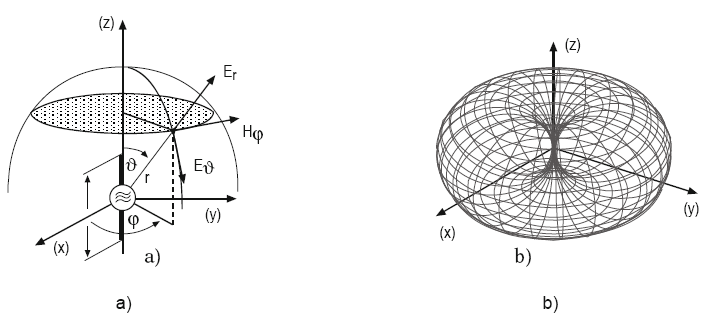
\includegraphics[width=.8\textwidth]{Abbildungen/Kapitel2/Feldverlauf.png}
    \caption[Darstellung der Feldvektoren eines Hertz'schen Dipoles und idealisierter Feldverlauf nach Quelle~\cite{EM_Schirmung}]{Darstellung der Feldvektoren eines Hertz'schen Dipoles in Kugelkoordinaten und idealisierte Darstellung der Feldumgebung ausgehend vom Ursprung nach Quelle~\cite{EM_Schirmung}}
    \label{fig:2_Feldverlauf}
\end{figure}

Für die Amplituden der Feldvektoren, die im Allgemeinen komplex sind, lassen sich demnach folgende Ausdrücke bestimmen \cite{Antenna_Theory}, \cite{EMV}.

\begin{subequations}
\label{eq:2_elektrische_Feldvektoren}
    \begin{align}
        E_r &= \frac{\hat i l \sqrt{\frac{\mu_0}{\varepsilon_0}} \lambda \cos{\theta}}{j 4 \pi^2 r^3}\left(1+ j\frac{2\pi}{\lambda}r\right)e^{-j\frac{2\pi}{\lambda}r} \label{subeq:2_E-Feld1} \\
        E_\phi &= 0 \label{subeq:2_E-Feld2} \\
        E_{\theta} &= \frac{\hat i l \sqrt{\frac{\mu_0}{\varepsilon_0}} \lambda \sin{\theta}}{j 8 \pi^2 r^3}\left(1+ j\frac{2\pi}{\lambda}r + \left(j\frac{2\pi}{\lambda}r\right)^2\right)e^{-j\frac{2\pi}{\lambda}r} \label{subeq:2_E-Feld3}
    \end{align}
\end{subequations}

\begin{subequations}
\label{eq:2_magnetische_Feldvektoren}
    \begin{align}
        H_r &= 0 \hphantom{\text{DiesIstEinLangesPlatzhalterwort1111111111}} \label{subeq:2_H-Feld1}\\
        H_{\phi} &= \frac{\hat i l \sin{\theta}}{4 \pi r^2}\left(1+j\frac{2\pi}{\lambda}r\right)e^{-j\frac{2\pi}{\lambda}r} \label{subeq:2_H-Feld2}\\
        H_{\theta} &= 0
    \end{align}
\end{subequations}

Die \Gleichungen \eqref{eq:2_elektrische_Feldvektoren},~\eqref{eq:2_magnetische_Feldvektoren} sind im gesamten Gebiet bis auf die Quelle selbst gültig \cite{Antenna_Theory}. Mit ihnen lassen sich Interpretationen bezüglich der Eigenschaften einer Antennenumgebung vornehmen:
\par
\vspace{\linespace}
Bei Abständen $r< \lambda / 2\pi$ beginnen die Terme höherer Ordnung zu dominieren. Diese Umgebung wird als Nahfeld bezeichnet und bei der dort befindlichen Energie handelt es sich hauptsächlich um imaginäre, d.h. gespeicherte Energie \cite{Antenna_Theory}. Das Nahfeld kann nach~\cite{Bundesnetzagentur_Glossar_Nahfeld} weiterhin in reaktives und strahlendes Nahfeld, auch als Übergangsfeld bezeichent, unterteilt werden. Für Antennen beliebiger Bauart kann als Grenze zwischen dem reaktiven und dem strahlenden Nahfeld (Fresnel Region) der Abstand $r=0,62 \sqrt{D^3\lambda}$ angesehen werden, wobei $D$ die größte Ausdehnung der Antenne ist \cite{Antenna_Theory}. Im Nahbereich weist das elektrische Feld die beiden Komponenten $E_r$ und $E_{\theta}$ auf. $E_\theta$ und $H_\phi$ sind um \SI{90}{\degree} gegeneinander phasenverschoben~\cite{EM_Schirmung}. Vereinfacht man die Gleichungen unter Vernachlässigung der Terme niedriger Ordnung weisen diese Ähnlichkeit mit Gleichungen eines statischen Dipols auf, sodass im Nahfeldbereich auch von quasiststischen Feldern gesprochen wird. Je nach Antennenbauform kann das elektrische oder magnetische Feld in diesem Bereich überwiegen~\cite{EMV}. 
\par
\vspace{\linespace}
Unabhängig von der Antennenbauart herrscht in großen Abstand von der Antenne ein elektromagnetisches Wellenfeld, das sogenannte Fernfeld. In der Entfernung $r\gg \lambda / 2\pi$ können in den Gleichungen \eqref{eq:2_elektrische_Feldvektoren},~\eqref{eq:2_magnetische_Feldvektoren} die Terme höherer Ordnung vernachlässigt werden. Dabei wird ersichtlicht, dass die Komponente $E_r$ gegenüber $E_\theta$ von niedrigerer Potenz ist und somit in Näherung ebenfalls vernachlässigt werden kann. Somit sind in diesem Bereich nur $E_\theta$ und $H_\phi$ existent. Die beiden Komponenten des elektrischen und magentischen Feldes sind orthogonal zueinander und bilden Transversalelektromagnetische Wellen (TEM). Die Schwingung beider Feldkomponenten erfolgt gleichphasig, sodass das Verhältnis beider Größen im Raum und zeitlich konstant bleibt \cite{EMV}

\begin{equation}
    \frac{E_{\theta}}{H_{\phi}} = Z_0 = \sqrt{\frac{\mu_0}{\varepsilon_0}} = \pi \cdot \SI{120}{\ohm} \approx \SI{377}{\ohm}
\end{equation}

Der Widerstand $Z_0$ wird auch als Feldwellenwiderstand des freien Raumes bezeichnet und ist nur abhängig vom umgebenden Medium~\cite{EMV}. Der Wellenwiderstand $Z$ kann auch formal im Nahfeldbereich aus den Feldvektoren gebildet werden und ist im Allgemeinen eine komplexe Größe.
\par
\vspace{\linespace}
Während der Feldwellenwiderstand, über den die elektrischen und magnetischen Felder miteinander gekoppelt sind, unabhängig der verwendeten Antenne im Fernfeld konstant ist, unterscheiden sich die Verhältnisse der Feldstärken im Nahfeld in Abhängigkeit der Antennenbauart. Hochohmige Nahfelder, welche zum Beispiel Stabantennen umgeben, sind überwiegend elektrischer Natur, während niederohmige Felder von bspw. Rahmenantennen im Vergleich höhere magnetische Feldstärken im Nahfeldbereich aufweisen. In Abhängigkeit des Abstandes zu den Antennen fällt bzw. steigt der Betrags des Feldwellenwiderstandes und nähert sich dem Feldwellenwiderstand des freien Raumes $Z_0$ (siehe \Abb \ref{fig:2_Feldwellenwiderstand}). Für beliebige Antennen wird oft der Abstand $r\geq 2 D^2 / \lambda$ als obere Grenze für das strahlende Nahfeld und damit für den Beginn des Fernfeldes (Fraunhofer Region) genutzt~\cite{Antenna_Theory}.  


\begin{figure}[ht]
    \centering
    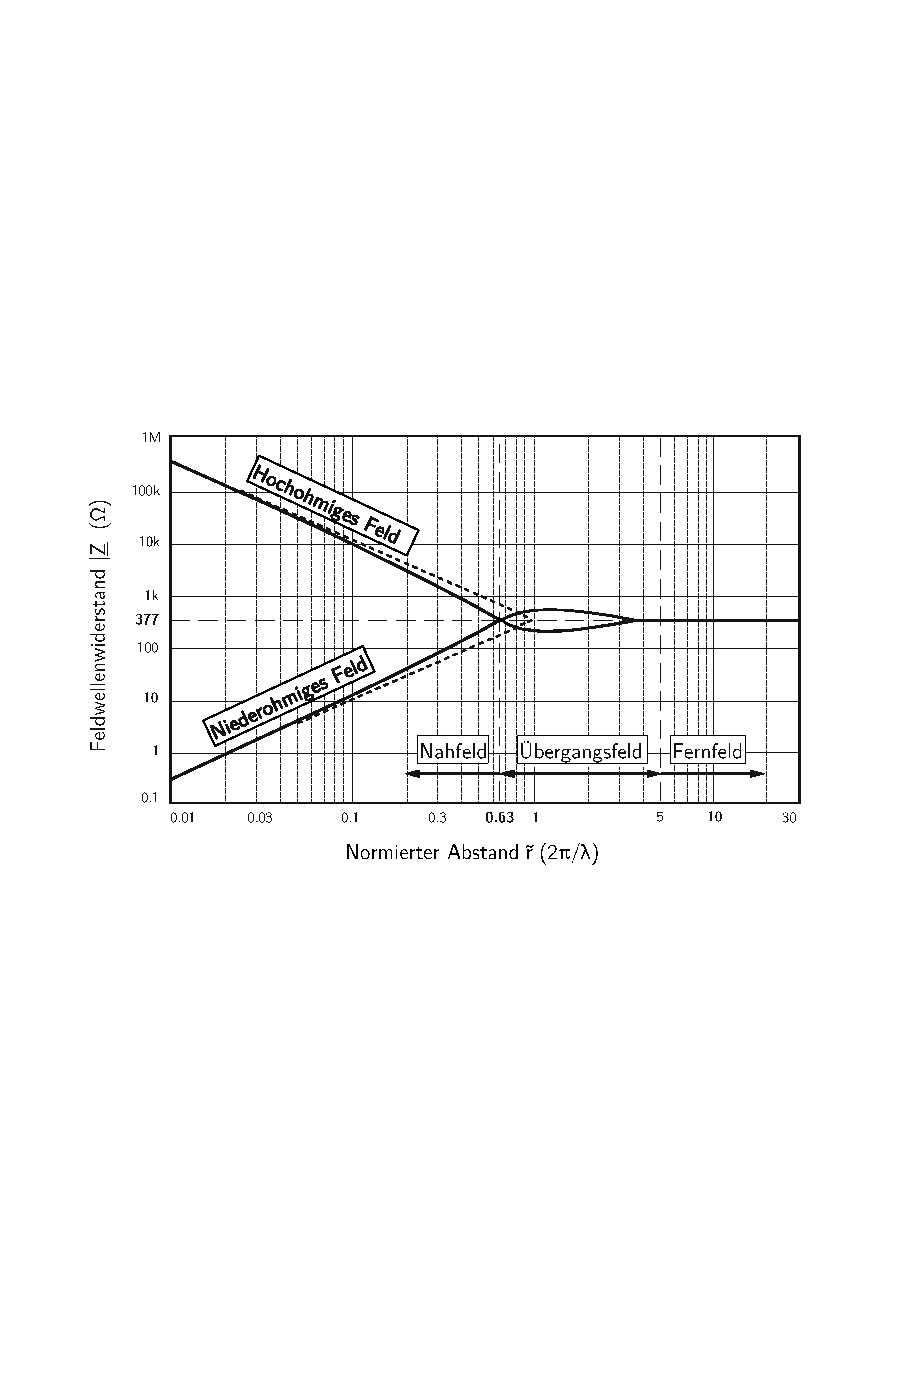
\includegraphics[page=1, width=0.8\textwidth, trim = 1.3cm 8.5cm 1.5cm 7cm, clip]{Abbildungen/Kapitel2/Feldwellenwiderstand.pdf}
    \caption{Verläufe des Feldwellenwiderstandes hoch- und niederohmiger Felder von Stab- und Rahmenantennen in Abhängigkeit des normierten Abstandes von der Feldquelle nach Quelle:~\cite{EMV}}
    \label{fig:2_Feldwellenwiderstand}
\end{figure}


Abhängig von der Art des vorliegenden Feldes unterscheiden sich die Maßnahmen zur Dämpfung und Schirmung maßgeblich voneinander, worauf in den folgenden Abschnitten näher eingegangen wird. Die Abhängigkeit der Natur des vorliegendes Feld, d.h. ist das Feld vorwiegend elektrisch oder magnetisch, in der Nähe einer Antenne von ihrer Bauform ist ebenfalls für Messungen relevant. Für niederfrequente Wechselfelder muss zwischen der Messung elektrischer Felder mit Stabantennen und magnetischer Felder mit Rahmenantennen unterschieden werden. Ab etwa \SI{30}{\mega\hertz} ist die Natur des zu vermessenden Feldes unerheblich für die Bauart der Messantenne, da sich bereits nach kurzem Abstand von der Quelle ein ebenes Wellenfeld ausbildet~\cite{Design_of_shielded_enclosures}.



\subsection{Dämpfung und Absorption}\label{cha:2_sub_Daempfung_und_Absorption}
In verlustbehafteten Medien tritt generell eine Dämpfung der elektrischen und magnetischen Feldstärke einer sich im Medium ausbreitenden Welle auf. Absorption bezeichnet eine sehr starke Dämpfung, wobei die Energie der Welle fast vollständig in Wärme umgesetzt wird. Bei einer von der Frequenz abhängigen Dämpfung wird außerdem die Form der Welle verändert, was als Dispersion bezeichent wird. 
\par
\vspace{\linespace}
Bei der Herleitung der Wellengleichung in Medien endlicher Leitfähigkeit $\sigma > 0$ (siehe \Anhang \ref{Anhang:Herleitung_Wellengleichung}) kann als Abkürzung der Darstellung die komplexe Wellenzahl $k$

\begin{equation}
    k = \sqrt{\varepsilon \mu \omega^2 - j \omega \sigma \mu}
\end{equation}

eingeführt werden. Je größer der Imaginärteil von k, desto größer wird auch die Phasenverschiebung zwischen den elektrischen und magnetischen Feldgrößen~\cite{EM_Schirmung}. Daher bietet sich eine Zerlegung in Real- und Imaginärteil von k an

\begin{equation}
    k = \beta - j \alpha \quad \Leftrightarrow \quad jk = \alpha + j\beta \; ,
\end{equation}

wodurch man die Dämpfungskonstante $\alpha$ und die Phasenkosntante $\beta$ erhält. Diese können wiederum aus $k$ zu

\begin{align}
    \alpha &= \omega \sqrt{\frac{\varepsilon \mu}{2}} \sqrt{\sqrt{1+\left(\frac{\sigma}{\omega\varepsilon}\right)^2}-1} \\
    \beta &= \omega \sqrt{\frac{\varepsilon \mu}{2}} \sqrt{\sqrt{1+\left(\frac{\sigma}{\omega\varepsilon}\right)^2}+1}
\end{align}

bestimmt werden. Mit diesen Koeffizienten kann eine Interpretation der gewünschten Materialeigenschaften für Dämpfungselemente erfolgen. 
\par
\vspace{\linespace}
Für eine möglichst hohe Dämpfung muss $\alpha$ maximal werden. Dies kann durch eine hohe Leitfähigkeit $\sigma$ und hohe Permeabilität $\mu$ erreicht werden. Die Herausforderung ergibt sich jedoch dadurch, dass sich bei großer Änderung der Leitfähigkeit an einer Grenzfläche die Ausbreitungsbedingungen ggf. so stark ändern, dass die Welle nicht gedämpft, sondern reflektiert wird. Für Absorberelemente ist dies jedoch nicht gewünscht, sodass dort eine Dämpfung vor allem durch die Permeabilität erfolgt. Je nach Bauart und Einsatzfrequenz wird dabei dem Magnetfeld Energie durch Ummagnetisierung des Absorbers entzogen, wie es bei Ferritelementen der Fall ist, oder es wird aufgrund der Bauform und mäßiger Leitfähigkeit ein geringer Impdanzsprung hervorgerufen. Letzteres mit mit sogenannten Pyramidenabsorbern erreicht, die aus häufig graphitgetränktem \ac{PU} bestehen und damit ebenfall hochpermeabel sind~\cite{EM_Schirmung}. Je nach Frequenzbereich ist dabei die Höhe der Pyramidenelemente und damit der Winkel der Seitenflächen entscheident für die Absorptionswirkung bei möglichst geringer Reflektion. Je nach Einsatzzweck gibt es ebenfalls unterschiedliche Kombinationen auf Ferrit- und Pyramidenabsorbern, sowie andere Bauformen für spezielle Anwendungen~\cite{EMV-Support_Produktseite}, \cite{Telemeter_Produktseite}. Bei jeglicher Kombination mehrerer Absorber in Reihe entlang der Ausbreitungsrichtung der zu dämpfenden Welle muss wiederum darauf geachtet werden, dass die Leitfähigkeiten an der Grenzfläche möglichst genau übereinstimmen, um keinen Impedanzsprung hervorzurufen, der daraufhin im Sinne der Wellenausbreitung zu einer Grenzschicht führt, die ungewollte Reflektionen hervorruft. Diese Anpassung kann bei Pyramidenabsorbern bspw. durch den Anteil des Kohlenstoffs im Material geschehen~\cite{EM_Schirmung}.




\subsection{Reflektion}\label{cha:2_sub_Reflektion}


Für die Ausbreitung von Wellen im Raum müssen natürlich die im \Abschnitt \ref{cha:2_sub_Verhalten_an_Grenzflächen} vorgestellten Grenzflächen von Materialien einen erheblichen Einfluss haben. Da an der Grenzfläche die Bedingungen für die Feldvektoren \Gleichungen \eqref{eq:2_Flussdichtennormale} eingehalten werden müssen, muss zu einer durchgelassenen Teilwelle (Index \glqq$d$\grqq) stets eine reflektierte Teilwelle (Index \glqq$r$\grqq) hinzukommen, welche Bestandteil der Wellengleichung ist~\cite{EM_Schirmung}.
\par
\vspace{\linespace}
Für den Grenzfall einer idealleitenden Fläche, auf die eine ebene Wellen trifft, muss zum Beispiel die Tangentialkomponente der elektrischen Feldstärke verschwinden~\cite{EM_Schirmung}, was nach \Gleichung \eqref{subeq:2_Feldstaerketangentiale1} zu dem Schluss führt, dass auch die Tangentiale der einfallenden Welle verschwinden muss. Dies kann nur geschehen, indem sich beide gegenseitig vollständig auslöschen, was wiederrum nur bei vollständiger Reflektion geschehen kann.
\par
\vspace{\linespace}
Für eine detailliertere Betrachtung lassen sich zwei Fälle unterscheiden. Im Fall \uproman{1} ist das elektrische Feld parallel zur Einfallsebene, während es im Fall \uproman{2} senkrecht dazu steht (siehe \Abb \ref{fig:2_Wellenreflektion}). In der Darstellung ist die Zeichenebene die Einfallsebene. Da für die Betrachtung von TEM-Wellen und die Relektion an metallischen Oberflächen der Fall \uproman{2} relevant ist, soll hier nur dieser betrachtet werden~\cite{EM_Schirmung}.

\begin{figure}
    \centering
    \begin{subfigure}[c]{0.3\textwidth}
        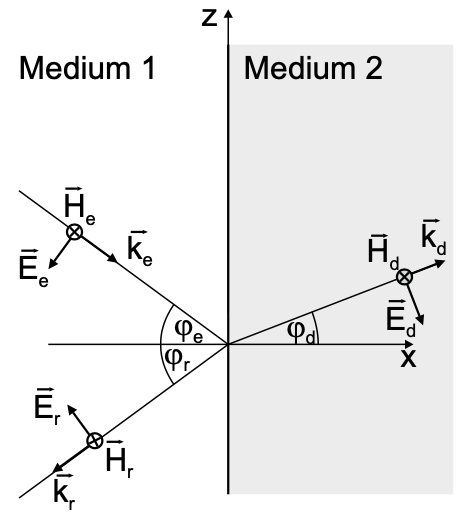
\includegraphics[width=\textwidth]{Abbildungen/Kapitel2/Wellenreflektion_Fall1.png}
        \caption{Fall \uproman{1}\label{subfig:2_Wellenreflektion_Fall1}}
    \end{subfigure}
    \hspace{0.2cm}
    \begin{subfigure}[c]{0.3\textwidth}
        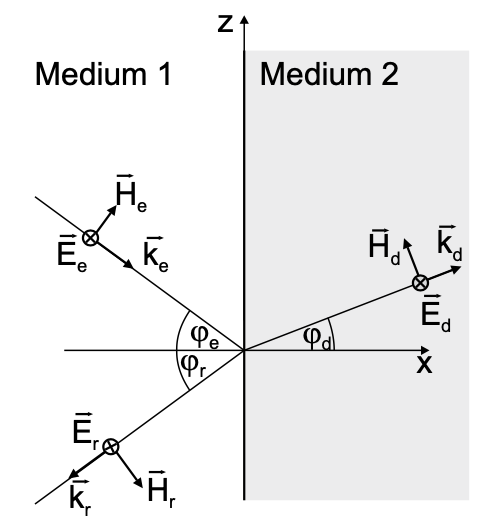
\includegraphics[width=\textwidth]{Abbildungen/Kapitel2/Wellenreflektion_Fall2.png}
        \caption{Fall \uproman{2}\label{subfig:2_Wellenreflektion_Fall2}}
    \end{subfigure}
    \caption[Schematische Darstellung des Auftreffens einer elektromagnetischen Welle auf eine Grenzfläche mit reflektierter und durchgelassener Teilwelle nach Quelle~\cite{EM_Schirmung}]{Schematische Darstellung des Auftreffens einer elektromagnetischen Welle auf eine Grenzfläche mit reflektierter und durchgelassener Teilwelle mit Fallunterscheidung entsprechend der Ausrichtung des elektrischen Feldes zur Einfallsebene (Darstellungsebene) nach Quelle~\cite{EM_Schirmung}.}
    \label{fig:2_Wellenreflektion}
\end{figure}

Für die Feldstärken gelten natürlich die Gleichungen~\eqref{eq:A_Wellengleichungen_mit_Leitfaehigkeit} aus der Herleitung der Wellengleichung im \Anhang \ref{Anhang:Herleitung_Wellengleichung}. Angewandt auf die dargestellten geometrischen Verhältnisse ergibt sich für die einfallende Welle (Index \glqq$e$\grqq)~\cite{EM_Schirmung}

\begin{align}
    \vec E_e &= E_0 e^{-j\vec k_e \vec r} \vec e_y \\
    \vec H_e &= \frac{E_0}{Z_1} \sin{\varphi_e} e^{-j \vec k_e \vec r} \vec e_x + \frac{E_0}{Z_1} \cos{\varphi_e} e^{-j \vec k_e \vec r} \vec e_z \\
    \vec k_e &= k_1 \cos{\varphi_e} \vec e_x - k_1 \sin{\varphi_e} \vec e_z \\
    Z_1 &= \frac{E_0}{H_0}
\end{align}

als Ausgangspunkt für die Betrachtung der Reflektion an einer Grenzfläche. Dabei ist zu berücksichtigen, dass hier die Ausbreitung, im Gegensatz zu \Gleichungen \eqref{eq:A_Wellengleichungen_mit_Leitfaehigkeit}, nicht in Richtung der x-Achse erfolgt, sondern entlang einer beliebigen Richtung. Dafür kann der Ortsvektor $\vec r$ als Ausgangspunkt und der Wellenzahlvektor $\vec k$ als Richtungsvektor mit
$|\vec k| = k = \sqrt{\varepsilon \mu \omega^2 - j \omega \sigma \mu} $ eingeführt werden~\cite{EM_Schirmung}. \par \vspace{\linespace} Analog kann für die reflektierte und die durchgelassene Teilwelle mit dem Reflektionsfaktor $R_{\uproman{2}}$ und dem Durchlassfaktor $D_{\uproman{2}}$

\begin{align}
    E_r &= E_0 R_{\uproman{2}} e^{-j\vec k_r \vec r} \vec e_y \\
    \vec H_r &= \frac{E_0}{Z_1} R_{\uproman{2}} \sin{\varphi_r} e^{-j \vec k_r \vec r} \vec e_x - \frac{E_0}{Z_1} R_{\uproman{2}} \cos{\varphi_r} e^{-j \vec k_r \vec r} \vec e_z \\
    \vec k_e &= - k_1 \cos{\varphi_r} \vec e_x - k_1 \sin{\varphi_r} \vec e_z \\
    E_d &= E_0 D_{\uproman{2}} e^{-j\vec k_d \vec r} \vec e_y \\
    \vec H_d &= \frac{E_0}{Z_2} D_{\uproman{2}} \sin{\varphi_d} e^{-j \vec k_d \vec r} \vec e_x + \frac{E_0}{Z_2} D_{\uproman{2}} \cos{\varphi_d} e^{-j \vec k_d \vec r} \vec e_z \\
    \vec k_d &= k_1 \cos{\varphi_d} \vec e_x - k_1 \sin{\varphi_d} \vec e_z
\end{align}

geschrieben werden. Unter Zuhilfenahme der Gesetzmäßigkeiten an Grenzflächen \Gleichungen \eqref{eq:2_Feldstaerketangentiale} für die Stelle $x=0$ lassen sich folgende Ausdrücke für den Reflektions- und den Durchlassfaktor finden, die das Verhältnis der beiden Teilwellen nach Auftreffen auf eine Grenzschicht beschreiben:

\begin{align}
    R_{\uproman{2}} &= \frac{Z_2 \cos{\varphi_e} - Z_1 \cos{\varphi_d}}{Z_2 \cos{\varphi_e} + Z_1 \cos{\varphi_d}} \\
    D_{\uproman{2}} &= \frac{2 Z_2 \cos{\varphi_e}}{Z_2 \cos{\varphi_e} + Z_1 \cos{\varphi_d}} \\ 
    1 &= D_{\uproman{2}} - R_{\uproman{2}} = D_{\uproman{2}} \frac{Z_1 \cos{\varphi_d}}{Z_2 \cos{\varphi_e}} + R_{\uproman{2}} \; .
\end{align}

Für den Fall, dass an der Grenzfläche kein Materialübergang stattfindet ($Z_1 = Z_2$), gilt $\varphi_e = \varphi_d$ und damit $R_{\uproman{2}} = 0$ und $D_{\uproman{2}} = 1$, das bedeutet die Welle wird nicht gebeugt und es findet keine Reflektions statt. Handelt es sich bei Medium 2 dagegen um einen idealen Leiter mit $Z_2 = 0 \neq Z_1$, so wird $D_{\uproman{2}} = 0$ und $R_{\uproman{2}} = -1$, was entsprechent der Erwartung heißt, dass eine eintreffende Welle an einer idealisierten metallischen Oberfläche vollständig reflektiert wird~\cite{EM_Schirmung}. 






